\chapter{Marco teórico}
\label{sec:teoria}

% Las figuras van con [H]: sin esto, una figura que pasa de página estira
% los espacios entre párrafos (marcoref.tex restaura \flushbottom al final).
\raggedbottom

% VERSIÓN DE PLANIFICACIÓN (19/10/2026): subtítulos e información por buscar.
% Cada sección se reemplaza por su redacción final.

\section{Estado del arte}
\label{sec:teoria_estado}

La revisión avanza desde las máquinas completas hacia los subsistemas. La
Sección~\ref{sec:teoria_dosificadoras} compara dosificadoras de ingredientes
secos, académicas y comerciales, y define la arquitectura funcional de
referencia. Las Secciones~\ref{sec:teoria_mecanica}
a~\ref{sec:teoria_control} analizan, por área, el almacenamiento y la
alimentación, la medición del peso y el control del corte, y cada una cierra
con los enfoques que se adoptan o se descartan. La
Sección~\ref{sec:teoria_fundamentos} reúne la teoría que aplica el diseño.

\section{Dosificadoras de ingredientes secos}
\label{sec:teoria_dosificadoras}

% Redacción del 20/10/2026, reorganizada según la plantilla (perspectivas
% académica y de mercado), THESIS_STRUCTURE y las referencias estructurales.
% Cifras verificadas con cada PDF o página. Moya, Lema, Acuña y Dargham
% pasan a la Sección 2.4.1 (principio de medición).

Esta sección revisa máquinas completas que dosifican ingredientes secos de
alimentos, primero desde la perspectiva académica y después desde la oferta
comercial. Los trabajos se ordenan desde la escala industrial hasta los equipos
más próximos a una panadería pequeña, y cada uno se valora por el dato técnico
que reporta, la limitación frente a la Panadería San Miguel y el criterio que
aporta al diseño. La revisión incluye dosificadoras de arroz, azúcar y otros
granos porque los trabajos con harina de trigo se limitan a consignas de
gramos. Esos equipos aportan la arquitectura, la escala de kilogramos y los
datos de error ausentes en la literatura de harina.

Las dosificadoras revisadas comparten la arquitectura funcional de la
Figura~\ref{fig:arquitectura_funcional}. La tolva almacena el ingrediente, el
alimentador lo entrega al recipiente de pesaje y la celda de carga mide la masa
acumulada. El controlador compara esa medición con la consigna y detiene el
alimentador para descargar el lote. En la figura, la línea continua sigue el
flujo de material y la línea discontinua, la información: la celda de carga
envía la señal de peso al controlador y este devuelve al alimentador el mando
de corte. Los antecedentes difieren en la forma de resolver cada bloque. La
tolva y el alimentador se analizan en la Sección~\ref{sec:teoria_mecanica}, el
pesaje en la Sección~\ref{sec:teoria_medicion} y el controlador en la
Sección~\ref{sec:teoria_control}.

\begin{figure}[H]
    \centering
    \resizebox{0.8\textwidth}{!}{\begin{tikzpicture}[
    >=Latex,
    font=\small,
    bloque/.style={
        rectangle,
        draw,
        rounded corners=2pt,
        minimum height=1.1cm,
        text width=2.7cm,
        align=center,
        inner sep=3pt
    },
    flecha/.style={
        -{Latex[width=6pt,length=5pt]},
        thick
    },
    senal/.style={
        -{Latex[width=6pt,length=5pt]},
        thick,
        dashed
    }
]

% Flujo de material
\node[bloque] (tolva) {Tolva de\\almacenamiento};
\node[bloque, right=0.9cm of tolva] (alim) {Alimentador};
\node[bloque, right=0.9cm of alim] (pesaje) {Recipiente de\\pesaje sobre\\celda de carga};
\node[bloque, right=0.9cm of pesaje] (descarga) {Descarga a la\\amasadora};

\draw[flecha] (tolva) -- (alim);
\draw[flecha] (alim) -- (pesaje);
\draw[flecha] (pesaje) -- (descarga);

% Control
\node[bloque, below=1.6cm of $(alim)!0.5!(pesaje)$] (ctrl) {Controlador};

\draw[senal] (pesaje.south) |- (ctrl.east);
\draw[senal] (ctrl.west) -| (alim.south);

\end{tikzpicture}
}
    \caption{Arquitectura funcional de una dosificadora gravimétrica por lotes.}
    \label{fig:arquitectura_funcional}
    \vspace{0.2em}
    {\footnotesize Fuente: Elaboración propia con base en las fuentes de la
    Sección~\ref{sec:teoria_dosificadoras}.}
\end{figure}

\subsection{Dosificadoras de granos y polvos}
\label{subsec:dosificadoras_academicos}

En la escala industrial, \textcite{gebov2023algorithmic} trabajó sobre
embolsadoras de sacos de 25~kg de harina con dosificador de tornillo y dos
celdas de carga. El método estima el instante de cierre mediante transformada
de Fourier y extrapolación de la señal de peso, y redujo el ciclo de 15 a 6~s
sin cambios en la mecánica. El trabajo confirma el pesaje gravimétrico de
harina en kilogramos, aunque con accionamiento trifásico y transporte de
envases ajenos a la carga por lotes de una amasadora.

En la escala de gramos, los prototipos comparten la arquitectura electrónica de
la Figura~\ref{fig:arquitectura_electronica}. La celda de carga entrega la
señal de peso a través del convertidor HX711, el microcontrolador la compara
con la consigna ingresada por teclado y acciona el motor del alimentador o el
servomotor de la compuerta, y la pantalla muestra la masa acumulada. Sobre esa
base común, los resultados varían con el tipo de alimentador.

\begin{figure}[H]
    \centering
    \resizebox{0.95\textwidth}{!}{\begin{tikzpicture}[
    >=Latex,
    font=\small,
    bloque/.style={
        rectangle,
        draw,
        rounded corners=2pt,
        minimum height=0.9cm,
        minimum width=3.4cm,
        text width=3.2cm,
        align=center,
        inner sep=3pt
    },
    grupo/.style={
        rectangle,
        draw,
        dashed,
        rounded corners=3pt,
        inner sep=7pt
    },
    titulo/.style={
        font=\footnotesize\bfseries,
        anchor=south
    },
    flecha/.style={
        -{Latex[width=6pt,length=5pt]},
        thick
    }
]

% Entradas (x = 0)
\node[bloque] (celda)     at (0, 1.8)  {Celda de carga};
\node[bloque] (hx)        at (0, 0.6)  {Convertidor HX711};
\node[bloque] (teclado)   at (0, -0.6) {Teclado o botones};
\node[bloque] (presencia) at (0, -1.8) {Sensor de presencia del recipiente};

% Procesamiento (x = 5)
\node[bloque, minimum height=3.3cm] (mcu) at (5, 0) {Microcontrolador\\(Arduino o ESP32)};

% Salidas (x = 10 y 14)
\node[bloque] (driver) at (10, 1.2)  {Controlador de motor};
\node[bloque] (alim)   at (14, 1.2)  {Motor del tornillo o del vibrador};
\node[bloque] (servo)  at (10, 0)    {Servomotor de la compuerta};
\node[bloque] (lcd)    at (10, -1.2) {Pantalla LCD};

% Conexiones
\draw[flecha] (celda) -- (hx);
\draw[flecha] (hx.east) -- (hx.east -| mcu.west);
\draw[flecha] (teclado.east) -- (teclado.east -| mcu.west);
\draw[flecha] (presencia.east) -- ++(0.6,0) |- ([yshift=0.35cm]mcu.south west);
\draw[flecha] (mcu.east |- driver.west) -- (driver.west);
\draw[flecha] (driver) -- (alim);
\draw[flecha] (mcu.east |- servo.west) -- (servo.west);
\draw[flecha] (mcu.east |- lcd.west) -- (lcd.west);

% Agrupaciones
\begin{scope}[on background layer]
    \node[grupo, fit=(celda)(presencia)] (gin) {};
    \node[grupo, fit=(mcu)] (gproc) {};
    \node[grupo, fit=(driver)(alim)(lcd)] (gout) {};
\end{scope}
\node[titulo] at (gin.north) {Entradas};
\node[titulo] at (gproc.north) {Procesamiento};
\node[titulo] at (gout.north) {Salidas};

\end{tikzpicture}
}
    \caption{Arquitectura electrónica de los prototipos de dosificación de bajo costo.}
    \label{fig:arquitectura_electronica}
    \vspace{0.2em}
    {\footnotesize Fuente: Elaboración propia con base en
    \textcite{david2024granulated}, \textcite{valendi2025granule},
    \textcite{orozco2024dosificadora} y
    \textcite{humaira2024optimalisasi}.}
\end{figure}

Con bandeja vibratoria,
\textcite{valendi2025granule} registraron errores promedio de 0,255 a 0,5~\% en
arroz de 50 a 400~g, con el menor error en la velocidad media del vibrador. Con
transportador de tornillo, \textcite{david2024granulated} obtuvieron
exactitudes de 99,677 a 99,795~\% para 120 a 175~g de azúcar, arroz y café,
mientras que \textcite{zaenurrohman2023merica} registraron un error promedio de
2,78~\% con pimienta en polvo, el material más fino del grupo. Estos trabajos validan una
arquitectura de bajo costo con errores de 0,2 a 2,8~\%, aunque
\textcite{david2024granulated} reconocen una capacidad limitada de adaptación
ante cambios de densidad o humedad del material.

En la escala de kilogramos, la más próxima al caso, predominan los ensayos con
granos. La electrónica se mantiene, con microcontrolador y convertidor HX711
\parencite{andriani2022rice,hadi2025weighing}, y la diferencia aparece en el
material que sigue cayendo después del cierre. \textcite{andriani2022rice}
dosificaron de 1 a 5~kg de arroz con una exactitud cercana al 95~\% y
atribuyeron la diferencia al arroz que cae tras el cierre de la válvula.
\textcite{hadi2025weighing} compensaron ese material con un adelanto de corte
de 120~g y registraron un sobrepaso promedio de 0,72~\% en cargas de 1 a
20~kg, con un servomotor en lugar de la válvula neumática industrial.
\textcite{bulatov2021dosing} trabajaron con harina de madera, el polvo más
próximo a la harina entre estos trabajos. Un variador de frecuencia reduce la
velocidad del tornillo en el tramo final del lote, el programa descuenta de
0,1 a 0,5~kg de material en caída y el error no superó el 5~\% en lotes de
1~kg, mientras que las virutas formaron bóvedas y no pudieron dosificarse. Con
alimentos en polvo, \textcite{ekpu2023weighing} reportaron una exactitud
aproximada del 95~\% y dosificaron 4,82~kg en 300~s.

La Figura~\ref{fig:secuencia_llenado} resume la secuencia de llenado que
resulta de estos trabajos. La masa crece rápido durante el flujo grueso y, al
acercarse a la consigna, el alimentador pasa a flujo fino. El corte se ordena
antes de la consigna, con un adelanto igual a la masa que aún está en caída,
y ese material completa el lote. La línea punteada muestra el caso sin
adelanto, en el que el material en caída produce el exceso que reportaron
\textcite{andriani2022rice}.

\begin{figure}[H]
    \centering
    \resizebox{0.7\textwidth}{!}{\begin{tikzpicture}[
    >=Latex,
    font=\small,
    eje/.style={-{Latex[width=5pt,length=5pt]}, thick},
    curva/.style={very thick},
    guia/.style={densely dashed, gray},
    nota/.style={font=\footnotesize, align=center}
]

% Ejes
\draw[eje] (0,0) -- (12.2,0) node[below left] {Tiempo};
\draw[eje] (0,0) -- (0,5.6) node[above right] {Masa en el recipiente};

% Consigna y masa de corte
\draw[guia] (0,4.0) -- (12,4.0);
\node[nota, anchor=east] at (0,4.0) {Consigna};
\draw[guia] (0,3.3) -- (7.5,3.3);
\node[nota, anchor=east] at (0,3.3) {Corte};

% Cambio de flujo y corte
\draw[guia] (4.5,0) -- (4.5,2.6);
\draw[guia] (7.5,0) -- (7.5,3.3);
\node[nota] at (2.25,0.45) {Flujo grueso};
\node[nota] at (6.0,0.45) {Flujo fino};
\node[nota] at (9.4,0.45) {Material en caída};

% Llenado con corte anticipado
\draw[curva] (0,0) -- (4.5,2.6) -- (7.5,3.3)
    .. controls (8.0,3.6) and (8.4,4.0) .. (9.0,4.0) -- (12,4.0);

% Llenado sin corte anticipado
\draw[thick, dotted] (7.5,3.3) -- (10.5,4.0)
    .. controls (10.9,4.3) and (11.2,4.7) .. (12,4.7);
\node[nota, anchor=south] at (10.9,4.8) {Sin adelanto: sobrepaso};

% Adelanto de corte
\draw[{Latex[width=4pt,length=4pt]}-{Latex[width=4pt,length=4pt]}]
    (7.2,3.3) -- (7.2,4.0);
\node[nota, anchor=south east] at (7.3,4.05) {Adelanto de corte};

\end{tikzpicture}
}
    \caption{Secuencia de llenado con flujo grueso, flujo fino y corte anticipado.}
    \label{fig:secuencia_llenado}
    \vspace{0.2em}
    {\footnotesize Fuente: Elaboración propia con base en
    \textcite{andriani2022rice}, \textcite{hadi2025weighing} y
    \textcite{bulatov2021dosing}.}
\end{figure}

Los trabajos de grado latinoamericanos ensayaron dosis de hasta 2~kg.
\textcite{orozco2024dosificadora} construyó una dosificadora de arroz por
ganancia de peso con canal vibratorio, compuerta y celda de carga de 10~kg
(Figura~\ref{fig:orozco_dosificadora}). La exactitud fue de 98,47~\% en 100
pruebas de 1~lb y de 99,73~\% en 30 pruebas de 1~kg, con 35,86~s por
kilogramo. \textcite{remache2022dosificador} dosificó cebada con tornillo de
0,1 a 2~kg, con un error relativo de hasta 10~\% en 0,1~kg y una diferencia
máxima de 0,013~kg. Ambos coinciden en que el error crece al disminuir la
dosis.

\begin{figure}[H]
    \centering
    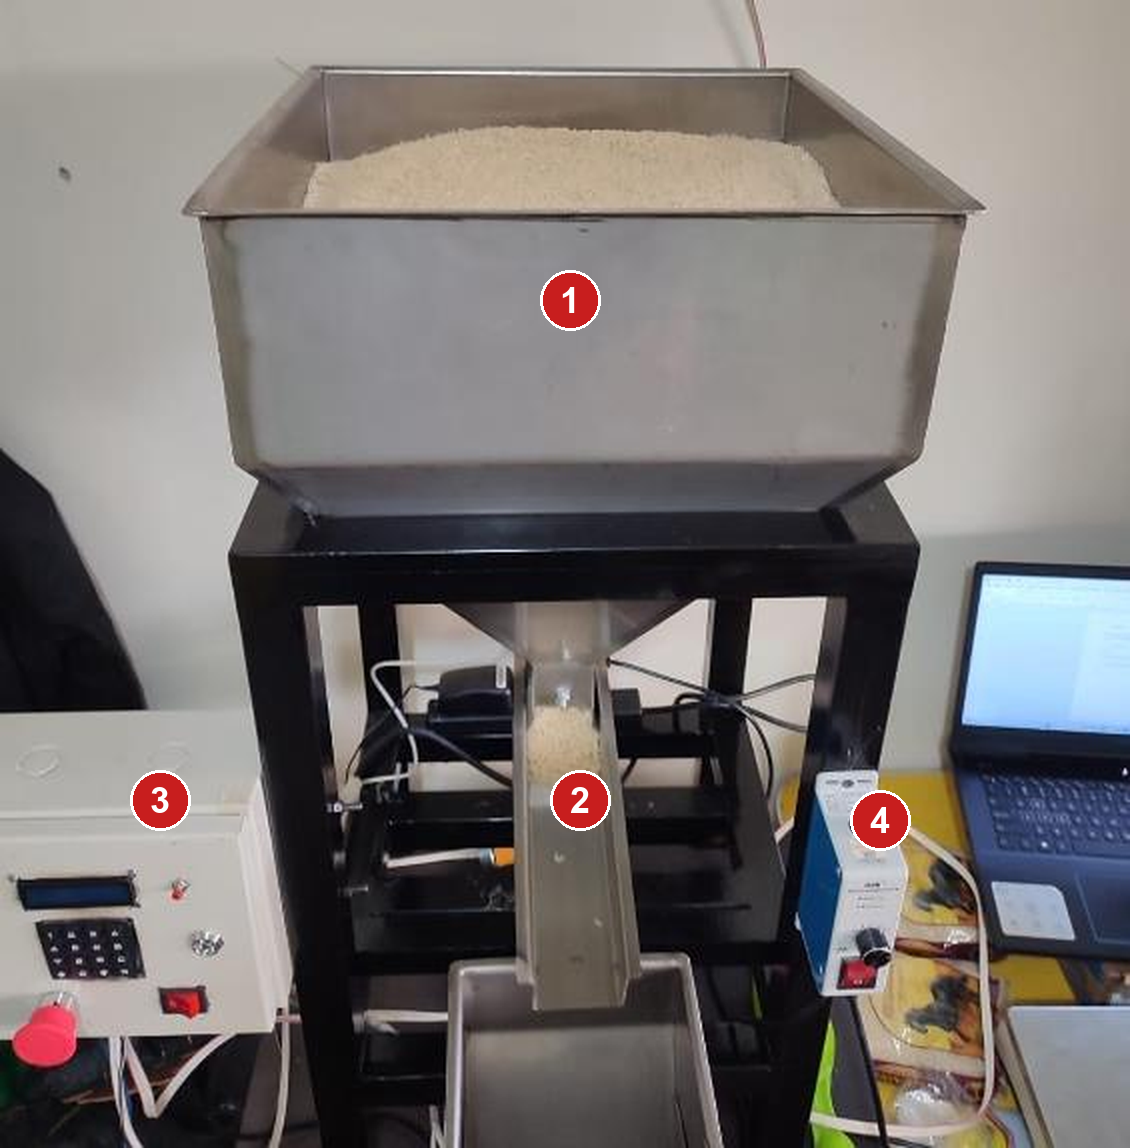
\includegraphics[width=0.45\textwidth]{images/marcoteorico/orozco_dosificadora.png}
    \caption{Dosificadora de arroz para microempresas con canal vibrante.}
    \label{fig:orozco_dosificadora}
    \vspace{0.2em}
    {\footnotesize 1: tolva, 2: canal vibrante, 3: gabinete de control,
    4: control de voltaje del canal.\\
    Fuente: Adaptado de \textcite{orozco2024dosificadora}.}
\end{figure}

\textcite{hidalgo2020llenado} diseñó una llenadora de granola con
tornillo y celda de carga en lazo cerrado, cuya prueba de concepto redujo el
tiempo de llenado en más del 40~\%, y recomienda separar el ajuste grueso del
fino. En Bolivia, \textcite{laime2022dosificacion} construyó un sistema para
snacks con canales vibratorios y tolvas de pesaje de 2,5~kg, y
\textcite{challco2024dosificadora} y \textcite{murillo2024papas} diseñaron
dosificadoras con celda de carga para pan molido y papas fritas. Estos tres
trabajos muestran que la dosificación por peso se estudia en el país, aunque
sin ensayos con harina y, en los dos últimos, sin resultados medidos.

\subsection{Dosificadoras para panadería}
\label{subsec:dosificadoras_panaderia}

Los trabajos más próximos al caso dosifican insumos de panadería.
\textcite{farihin2021premix} dosificaron una premezcla de pan dulce desde cinco
tolvas hacia una única celda de carga de 1~kg, y el control PI registró un
error de 0,2~\%, frente a 0,8~\% con control todo o nada.
\textcite{humaira2024optimalisasi} emplearon, en cambio, tres cámaras para
harina, leche en polvo y azúcar, cada una con alimentador helicoidal y celda de
carga propia (Figura~\ref{fig:humaira_dosificadora}), y lograron un error
promedio de 0,08~\% en harina con 197~s para 350~g.

\begin{figure}[H]
    \centering
    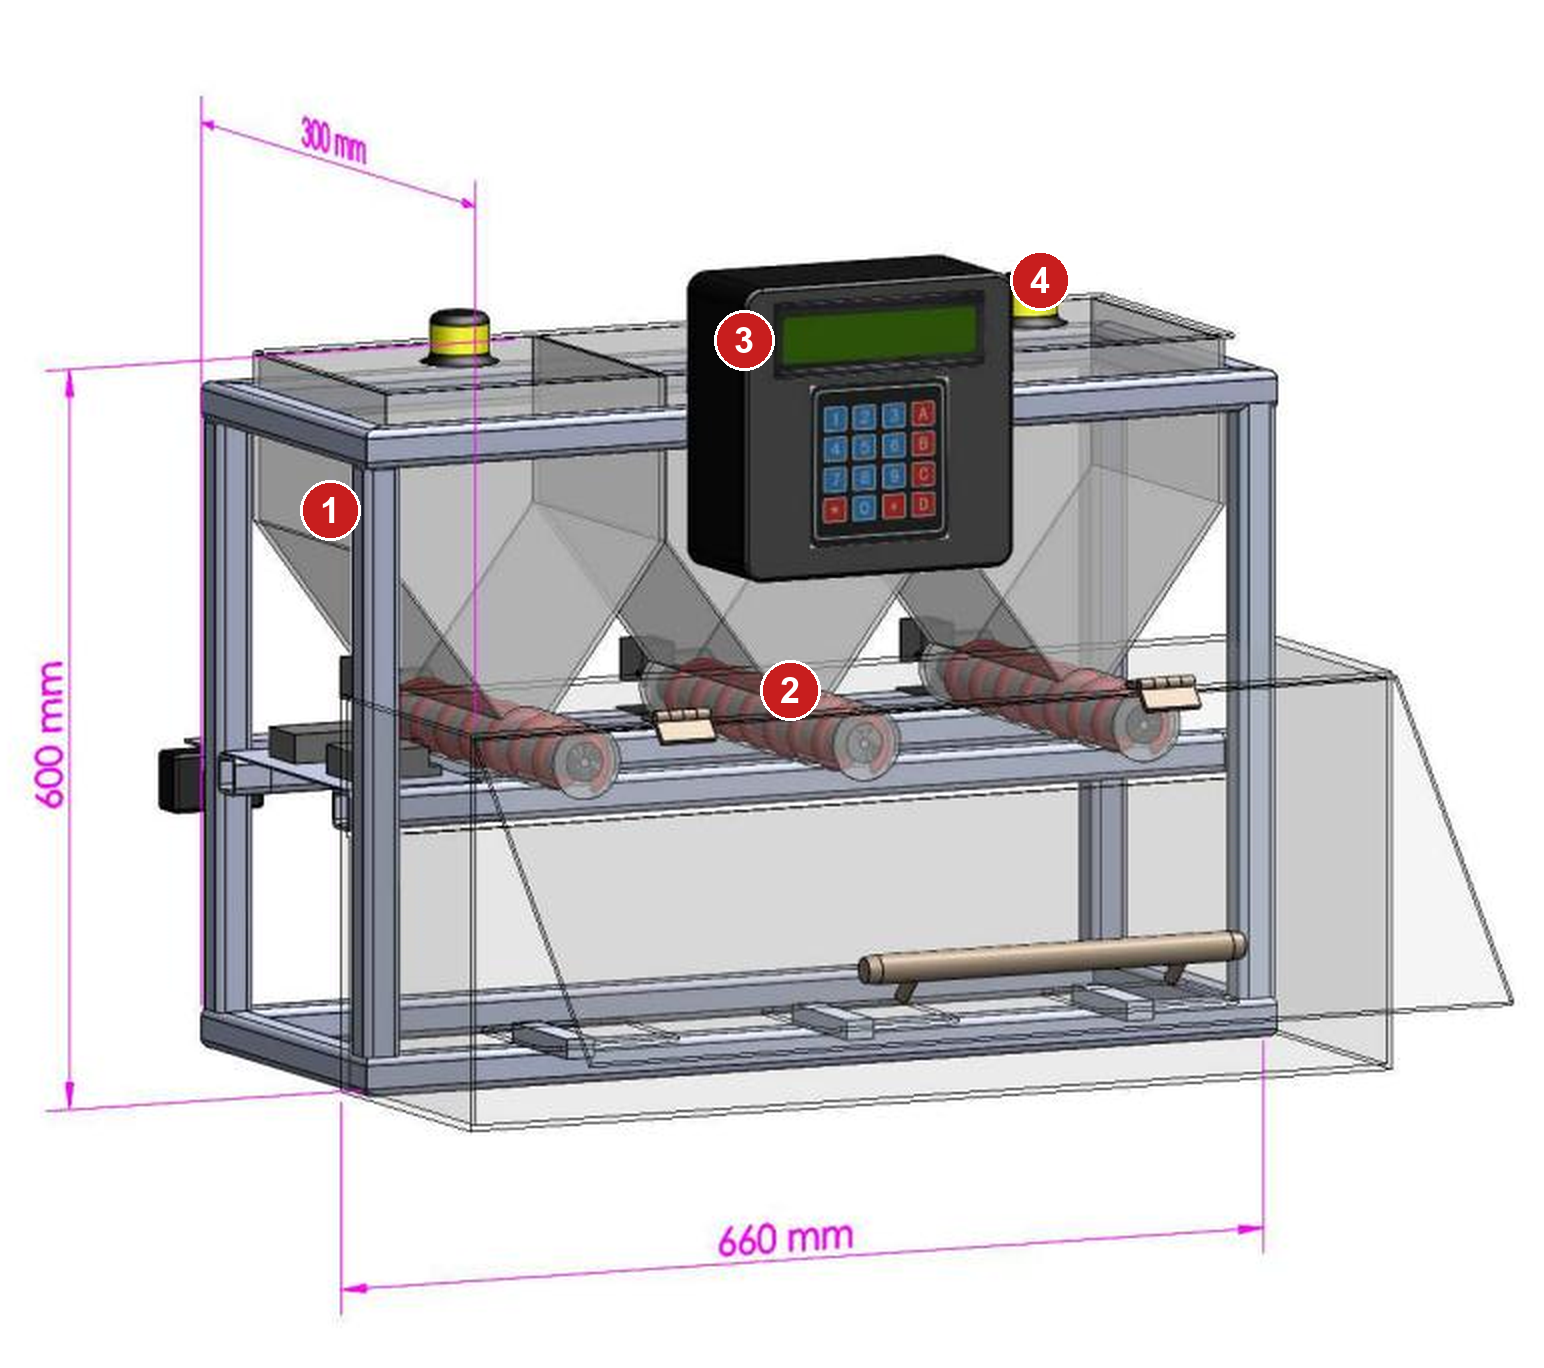
\includegraphics[width=0.6\textwidth]{images/marcoteorico/humaira_dosificadora.png}
    \caption{Dosificadora de insumos para pan con tres cámaras y alimentadores helicoidales.}
    \label{fig:humaira_dosificadora}
    \vspace{0.2em}
    {\footnotesize 1: cámara de insumo, 2: alimentador helicoidal, 3: caja con
    pantalla y teclado, 4: sensor infrarrojo de nivel.\\
    Fuente: Adaptado de \textcite{humaira2024optimalisasi}.}
\end{figure}

\textcite{rumapea2026flour} diseñaron una dosificadora de harina de trigo para
pequeñas panaderías con tolva cónica de acrílico, compuerta accionada por
servomotor y celda de carga de 1~kg. La compuerta permanece abierta hasta
el 90~\% de la consigna y pasa a flujo fino hasta el cierre, con un error
porcentual absoluto medio de 1,32 a 1,83~\% en 30 ensayos por consigna de 10 a
50~g. El ensayo de mayor error entregó 47,40~g para 50~g, y los autores lo
atribuyen a una bóveda de harina en el borde de la compuerta.
\textcite{bachtiar2026brownies} integraron la dosificación y el mezclado de
masa para brownies en un mismo equipo, con seis compuertas accionadas por
servomotor que vacían por turno los insumos secos sobre una sola celda de
carga. En la prueba de insumos, la harina de trigo llegó a 95~g frente a una
consigna de 100~g y el azúcar a 51~g frente a 120~g, y los autores concluyen
que la apertura por servomotor requiere mejoras para los insumos secos.

Humaira et al., Rumapea et al. y Bachtiar et al. son los únicos trabajos
revisados con ensayos en harina de trigo, con una consigna mayor de 350~g. De este grupo se toman
tres criterios. La bóveda condiciona el diseño de la tolva y del alimentador
(Sección~\ref{sec:teoria_mecanica}). El error menor del control PID se obtuvo
con el caudal menor, por lo que el tiempo por lote es una variable de diseño
junto con la exactitud. Los insumos admiten una balanza común con dosificación
secuencial \parencite{farihin2021premix,bachtiar2026brownies} o una balanza por insumo
\parencite{humaira2024optimalisasi}.

\subsection{Productos comerciales}
\label{subsec:dosificadoras_mercado}

La oferta para panificación industrial dosifica por peso y separa la harina de
los insumos menores. En la planta de Harry-Brot, AZO alimenta las amasadoras
con básculas de vacío para la harina y pesa los insumos menores al gramo en
balanzas propias, con fondos vibratorios y tornillos de dosificación
fina~\parencite{azo2026kneader}. El sistema MicDos de Zeppelin dosifica hasta
20 componentes con tornillo y variador de frecuencia, flujo grueso y fino y
corrección del sobrepaso, sobre una balanza móvil de
25~kg~\parencite{zeppelin2026micdos}. La industria aplica, por tanto, el corte
en dos etapas con compensación del material en caída. En Latinoamérica, INOXPA
instaló para un fabricante de pan una báscula sobre celdas de carga de 200~kg
con exactitud declarada del 1~\%, controlada por PLC y
SCADA~\parencite{inoxpa2026pastry}.

Para panaderías de menor tamaño, Daxner ofrece dosificación volumétrica o
gravimétrica y componentes para panaderías artesanales, sin especificaciones
publicadas~\parencite{daxner2026bakery}. El resto de la oferta revisada
corresponde a envasado o a dosificación continua. RUICHUAN vende unidades por
pérdida de peso~\parencite{UnidadDosificadoraGravimetrica}, y Trust-Long,
llenadoras semiautomáticas de polvo con tolvas de 20 y
50~L~\parencite{MaquinaLlenadoPolvo}. La oferta comercial confirma el principio
y la estrategia de corte, pero se orienta a plantas industriales o no publica
especificaciones para panaderías pequeñas. La comparación de costos
corresponde al análisis económico (Sección~\ref{subsec:justificacion_economica}).

\subsection{Enfoques adoptados y descartados}
\label{subsec:dosificadoras_enfoques}

La Tabla~\ref{tab:dosificadoras_resumen} reúne los trabajos que dosificaron
harina o masas del orden del kilogramo, con el insumo, la consigna, el
alimentador, el error y el caudal de cada uno. El error se presenta con la
métrica de cada autor, por lo que las cifras no se comparan directamente entre
filas. El caudal es un cálculo propio, la masa dosificada dividida entre el
tiempo reportado, y permite contrastar los prototipos con el ritmo de trabajo
de la panadería.

\begin{table}[htbp]
    \centering
    \caption{Dosificadoras de harina y de escala de kilogramos: error y caudal.}
    \label{tab:dosificadoras_resumen}
    \footnotesize
    \setstretch{1}
    \setlength{\tabcolsep}{3pt}
    \renewcommand{\arraystretch}{1.2}

    \begin{tabularx}{\textwidth}{
        >{\raggedright\arraybackslash}p{0.18\textwidth}
        >{\raggedright\arraybackslash}p{0.12\textwidth}
        >{\raggedright\arraybackslash}p{0.11\textwidth}
        >{\raggedright\arraybackslash}p{0.16\textwidth}
        >{\raggedright\arraybackslash}X
        >{\raggedright\arraybackslash}p{0.09\textwidth}}
        \toprule[1pt]
        \textbf{Fuente} & \textbf{Insumo} & \textbf{Consigna} &
        \textbf{Alimentación} & \textbf{Error según el autor} &
        \textbf{Caudal (kg/h)} \\
        \midrule[1pt]
        \textcite{gebov2023algorithmic} & Harina & 25~kg & Tornillo &
        No reporta & 6000 a 15\,000 \\
        \textcite{humaira2024optimalisasi} & Harina & 20--350~g & Helicoide &
        Error medio de 0,08~\% & 6 \\
        \textcite{rumapea2026flour} & Harina de trigo & 10--50~g & Compuerta &
        EPAM de 1,32 a 1,83~\% (n = 30) & --- \\
        \textcite{andriani2022rice} & Arroz & 1--5~kg & Válvula &
        Exactitud cercana al 95~\% & --- \\
        \textcite{hadi2025weighing} & Arroz & 1--20~kg & Válvula &
        Sobrepaso medio de 0,72~\% & --- \\
        \textcite{ekpu2023weighing} & Alimentos en polvo & 1~kg & Motor paso
        a paso & Exactitud cercana al 95~\% & 58 \\
        \textcite{bulatov2021dosing} & Harina de madera & 1~kg & Tornillo &
        Hasta 5~\% & --- \\
        \textcite{orozco2024dosificadora} & Arroz & 0,4~lb--1~kg & Canal
        vibratorio & Exactitud de 99,73~\% con 1~kg (n = 30) & 100 \\
        \textcite{remache2022dosificador} & Cebada & 0,1--2~kg & Tornillo &
        Hasta 10~\% con 0,1~kg, máximo de 0,013~kg & --- \\
        \bottomrule[1pt]
    \end{tabularx}

    \vspace{2pt}
    {\footnotesize EPAM: error porcentual absoluto medio. n: ensayos por
    consigna. Caudal: cálculo propio a partir de la masa y el tiempo
    reportados. ---: la fuente no reporta tiempo por dosis.
    Fuente: Elaboración propia con base en las fuentes citadas.}
\end{table}

Los prototipos con tiempo reportado alcanzan caudales de 6 a 100~kg/h. Como
referencia, el procedimiento manual de San Miguel registró de 5 a 8~kg en
ciclos de 53,2 a 66,6~s (Apéndice~\ref{ap:tablas_dosificacion}), equivalentes
a un intervalo aproximado de 270 a 540~kg/h. Este cálculo usa el tiempo total
del ciclo, que incluye acciones del operario, y no constituye un requisito.
Ningún prototipo alcanza ese orden de caudal, y el error menor en harina se
obtuvo con 6~kg/h \parencite{humaira2024optimalisasi}. Esa
brecha entre caudal y exactitud da relevancia al corte en dos etapas que aplica
la industria.

La Tabla~\ref{tab:dosificadoras_enfoques} contrasta los enfoques identificados
en la revisión. Cada fila corresponde a una alternativa para un bloque de la
Figura~\ref{fig:arquitectura_funcional}, el principio de medición, el
alimentador, la estrategia de corte o el número de balanzas, y presenta el
resultado que la favorece y la limitación observada, con el autor que la
reporta.

\begin{table}[H]
    \centering
    \caption{Factores a favor y limitaciones de los enfoques de dosificación.}
    \label{tab:dosificadoras_enfoques}
    \footnotesize
    \setstretch{1}
    \setlength{\tabcolsep}{3pt}
    \renewcommand{\arraystretch}{1.25}

    \begin{tabularx}{\textwidth}{
        >{\raggedright\arraybackslash}p{0.24\textwidth}
        >{\raggedright\arraybackslash}X
        >{\raggedright\arraybackslash}X}
        \toprule[1pt]
        \textbf{Enfoque} & \textbf{Factores a favor} & \textbf{Limitaciones} \\
        \midrule[1pt]
        Pesaje por lotes: tolva, alimentador, celda de carga y controlador &
        Errores de 0,2 a 2,8~\% en prototipos de bajo costo & Ensayos con
        granos y caudales de 6 a 100~kg/h \\
        Dosificación volumétrica & Sin celda de carga & Masa no medida, con
        evidencia en la Sección~\ref{sec:teoria_medicion} \\
        Pesaje industrial de sacos y envases & Ciclo de 6~s en sacos de 25~kg de harina (Gebov) &
        Accionamiento trifásico y transporte de envases \\
        Tornillo & 0,08~\% en harina (Humaira) y 99,68 a 99,80~\% (David) &
        6~kg/h en harina y bóvedas con virutas (Bulatov) \\
        Canal vibratorio & 0,255 a 0,5~\% (Valendi) y 99,73~\% con 1~kg
        (Orozco) & Ensayos con granos \\
        Compuerta & EPAM de 1,32 a 1,83~\% en harina (Rumapea) & Bóveda en el
        borde, material en caída (Andriani) y apertura poco controlable con
        insumos secos (Bachtiar) \\
        Corte en dos etapas, adelanto de corte o PID & Sobrepaso de 0,72~\%
        con adelanto de 120~g (Hadi) y flujo grueso y fino en la industria
        (Zeppelin) & 197~s para
        350~g con PID (Humaira) \\
        Balanza común o balanza por insumo & Una celda para cinco tolvas
        (Farihin) y balanzas separadas para insumos menores (AZO) & Sin
        comparación en un mismo trabajo \\
        Equipos comerciales & Principio y corte en dos etapas probados &
        Escala industrial o envasado \\
        \bottomrule[1pt]
    \end{tabularx}

    \vspace{2pt}
    {\footnotesize Fuente: Elaboración propia con base en las fuentes de la
    Sección~\ref{sec:teoria_dosificadoras}.}
\end{table}

A partir de la tabla, el proyecto adopta el pesaje por lotes con tolva,
alimentador, celda de carga y controlador como arquitectura de referencia,
porque reúne los menores errores con equipos de bajo costo. Se descarta la
dosificación volumétrica como principio, ya que no mide la masa entregada, y
se descarta la arquitectura de pesaje de sacos y envases, aunque se conserva su
principio gravimétrico. El tornillo, el canal vibratorio y la compuerta
presentan ventajas y fallas de flujo que dependen del material, por lo que su
selección se analiza en la Sección~\ref{sec:teoria_mecanica}, y las
estrategias de corte se comparan en la Sección~\ref{sec:teoria_control}. La
elección entre una balanza común y una balanza por insumo queda para el
diseño, porque ningún trabajo las compara, y los equipos comerciales sirven de
referencia técnica y económica.

Sin embargo, los ensayos con harina
de trigo se limitan a consignas de 10 a 350~g
\parencite{humaira2024optimalisasi,rumapea2026flour,bachtiar2026brownies}, los trabajos en el rango
de 5 a 8~kg emplean arroz \parencite{andriani2022rice,hadi2025weighing} y la
oferta comercial se orienta a plantas industriales o no publica especificaciones
para panaderías pequeñas. Ninguna de las fuentes
académicas revisadas reporta la dosificación gravimétrica de harina de trigo en
lotes de 5 a 8~kg, el intervalo medido en la Panadería San Miguel
(Apéndice~\ref{ap:tablas_dosificacion}). Ese intervalo, para una panadería
pequeña, define el aporte diferencial del proyecto.

\section{Área mecánica: almacenamiento y alimentación}
\label{sec:teoria_mecanica}

\subsection{Tolvas para polvos cohesivos}
Tolvas para harina y polvos cohesivos: formación de bóvedas, adherencia y
descarga.

\subsection{Alimentadores para dosificación por lotes}
Tornillo sin fin, alimentador vibratorio y otros: caudal, fallas de flujo y
limpieza.

\section{Área de medición: principio y sensores de peso}
\label{sec:teoria_medicion}

\subsection{Volumétrico frente a gravimétrico}
% Fuentes trasladadas desde 2.2 (20/10/2026): moya2016dosificador,
% lema2026dosificadora, acuna2024gravimetrico (sobreconsumo de 0,86 % con
% volumétricos de 10 g frente a 2 g gravimétrico) y dargham2025volumetric
% (la masa varía con la humedad porque el alimentador controla volumen).
% Pendiente: Chiliguana y Villavicencio (ESPOL, 2016, archivo D-CD88349.pdf),
% rediseño de dosificadora volumétrica a gravimétrica de galletas (sobredosis
% de 3552,5 kg/mes con el sistema volumétrico, solo diseño).
Dosificación volumétrica frente a gravimétrica; pesaje por lotes y pérdida de
peso.

\subsection{Celdas de carga en dosificadoras}
Celdas de carga y errores por vibración, impacto, ruido y temperatura.

\section{Área de control: corte y control de la dosificación}
\label{sec:teoria_control}

\subsection{Estrategias de corte}
Alimentación en dos etapas, corte con adelanto y compensación del material en
caída.

\subsection{Control realimentado}
PID, aprendizaje iterativo y pesaje dinámico.

\section{Fundamentos teóricos}
\label{sec:teoria_fundamentos}

\subsection{Metodología de diseño}

\subsection{Insumos y tolerancias de dosificación}
Propiedades de la harina, la sal, el azúcar y la levadura, y efecto de su
variación en la masa.

\subsection{Metrología y normativa de pesaje}
Vocabulario metrológico (VIM), OIML R~61, R~76 y R~60.

\subsection{Medición gravimétrica y celdas de carga}
Galga extensométrica, celda de carga y acondicionamiento de la señal.

\subsection{Almacenamiento y alimentación de sólidos a granel}
Flujo en tolvas y caudal en alimentadores de tornillo y vibratorios.

\subsection{Modelamiento dinámico y control}
Conceptos básicos de modelado y control PID.

\section{Conclusión del capítulo}
\label{sec:teoria_conclusion}

Enfoques adoptados y descartados, y aporte diferencial del proyecto.
